\documentclass{beamer}
 
% === DATA === (((
\title{\sc Ejercicio 13--4 \\ M. Spivak. Caluclus.}
\author{Por Erick I. Rodríguez Juárez.}
\institute{VALUAMI}
\date{Miércoles, 7 de Agosto, 2024.}
% )))

% === FONT === (((
% \setbeamerfont{normal text}{series= \ttfamily}
% \AtBeginDocument{\usebeamerfont{normal text}}
\usefonttheme{professionalfonts}
\usefonttheme{serif}
\usepackage{fontspec}
\setmainfont[
  BoldFont       = bodonibi,
	ItalicFont     = Century modern italic2.ttf,
	BoldItalicFont = bodonibi,
	SmallCapsFont  = lmromancaps10-regular.otf
]{Century_modern.ttf}
% )))

% === FONT IN MATH MODE === (((
\DeclareSymbolFont{italics}{\encodingdefault}{\rmdefault}{m}{it}
\DeclareSymbolFontAlphabet{\mathit}{italics}
\ExplSyntaxOn
\int_step_inline:nnnn { `A } { 1 } { `Z }
 {  \exp_args:Nf \DeclareMathSymbol{\char_generate:nn{#1}{11}}{\mathalpha}{italics}{#1} }
\int_step_inline:nnnn { `a } { 1 } { `z } {  \exp_args:Nf \DeclareMathSymbol{\char_generate:nn{#1}{11}}{\mathalpha}{italics}{#1}}
\ExplSyntaxOff
% )))

% === COMMANDS === (((
\hfuzz=5pt % size of boxes
\newcommand{\dis}{\displaystyle}
\renewcommand{\qed}{\hspace{0.5cm}\rule{0.16cm}{0.4cm}}
\newcommand{\operator}[1]{\mathop{\vphantom{\sum}\mathchoice
{\vcenter{\hbox{\huge $#1$}}}
{\vcenter{\hbox{\Large $#1$}}}{#1}{#1}}\displaylimits}
\newcommand{\suma}{\operator{
\includegraphics[scale=0.09]{IMAGES/PORTADA/Sigma.png}}}
% )))

% === BEAMER TEMPLATE === (((
% DESPLIEGUE EN VARIAS DIAPOSITIVAS.
% display un item a la vez
\beamerdefaultoverlayspecification{<+(1)->}
% TITULOS EN SMALL CAPS
\setbeamerfont{title}{family=\scshape\huge}
\setbeamerfont{frametitle}{family=\scshape\LARGE}
\setbeamerfont{section in head/foot}{size = \normalsize, family=\scshape}

% sin footline
\setbeamertemplate{footline}{}

% \setbeamerfont{block title}{series=\sc}
% \setbeamerfont{block body}{series=\ttfamily }
% enumerates sin shade
\setbeamertemplate{enumerate items}[circle] % esto lo estoy usando para los simbolos de enumeración.
\setbeamertemplate{itemize items}[circle] % esto lo estoy usando para los simbolos de itemize.
\setbeamertemplate{section in toc}[circle] % esto lo estoy usando para los simbolos de enumeración.

% quitar espacio
% \addtobeamertemplate{titleframe}{}{\vspace{-5mm}}
% \addtobeamertemplate{block begin}{\vskip - \bigskipamount}{}
% \addtobeamertemplate{block end}{}{\vskip - \smallskipamount}
% \addtobeamertemplate{block example begin}{\vskip - \bigskipamount}{}
% \addtobeamertemplate{block example end}{}{\vskip - \smallskipamount}
% \addtobeamertemplate{block definition begin}{\vskip - \bigskipamount}{}
% \addtobeamertemplate{block definition end}{}{\vskip - \smallskipamount}

% PARA VER SECCIONES HORIZONTALMENTE
\setbeamertemplate{headline}{
\leavevmode
\hbox{
\begin{beamercolorbox}[wd=1.02\paperwidth,ht=4ex,dp=2ex]{palette quaternary}
\insertsectionnavigationhorizontal{\paperwidth}{\hskip 0pt plus1filll}{\hskip 0pt plus1filll}
\end{beamercolorbox}
}
}
% SECCIONES EN PÁGINAS.
\setbeamerfont{section title}{parent=title}
\setbeamertemplate{section page}
{
    \begin{centering}
	    \begin{beamercolorbox}[wd= \linewidth ,sep=12pt,center]{secciones}
    \usebeamerfont{frametitle}\insertsection\par
    \end{beamercolorbox}
    \end{centering}
}
\AtBeginSection{\frame{\sectionpage}}
% NUMBERS IN BIBLIOGRAPHY.
% \setbeamertemplate{bibliography item}[text]
% )))

% === COLORS === (((
\beamertemplatenavigationsymbolsempty % for remove the nav. symb.
\mode<presentation>

\colorlet{maincolor}{purple}
\colorlet{titlecolor}{teal}

\setbeamercolor{alerted text}{parent=palette secondary, bg=green!50}
\setbeamercolor*{palette primary}{   fg=white     , bg=maincolor}
\setbeamercolor*{palette secondary}{ fg=black     , bg=titlecolor!40}
\setbeamercolor*{palette tertiary}{  fg=white , bg=}
\setbeamercolor*{palette quaternary}{fg=white     , bg=black!20!maincolor}

\setbeamercolor*{titlelike}{parent=palette tertiary}
\setbeamercolor{frametitle}{parent=palette primary}

\setbeamercolor*{separation line}{}
\setbeamercolor*{fine separation line}{}
\setbeamercolor{block body}{parent=normal text,use=block title,bg=titlecolor!15!white,fg=black}
\setbeamercolor{block title}{bg=titlecolor!90!blue,fg=white}

\setbeamercolor{block title example}{bg=maincolor!80!black,fg=white}
\setbeamercolor{block body example}{bg=maincolor!15!white,fg=black}
\setbeamercolor{item projected}{bg=maincolor}

\setbeamercolor{section title}{parent=titlelike}
\setbeamercolor{secciones}{fg=black,bg=titlecolor!20}
\setbeamercolor{section in head}{parent=palette quaternary}
\setbeamertemplate{section in head/foot shaded}{\color{black!70!maincolor}\usebeamertemplate{section in head/foot}}
\mode<all>
% )))

% === TITLEPAGE === (((
\setbeamercolor{author}{fg = white}
\setbeamercolor{institute}{fg = white}
\setbeamercolor{date}{fg = white}
\newcommand{\portada}{
{
\addfontfeature{LetterSpace=-5}
\usebackgroundtemplate{
\includegraphics[width=  \paperwidth]{IMAGES/PORTADA/purple_teal.pdf}}
\begin{frame}[plain]
\titlepage
\end{frame}
}
}
% )))

\begin{document}

\portada

\section[Enunciado]{Ejercicio 13--4. Spivak} % (((
% \frame{\sectionpage}
\begin{frame}[t]
	\frametitle{\secname}
	\centering 
	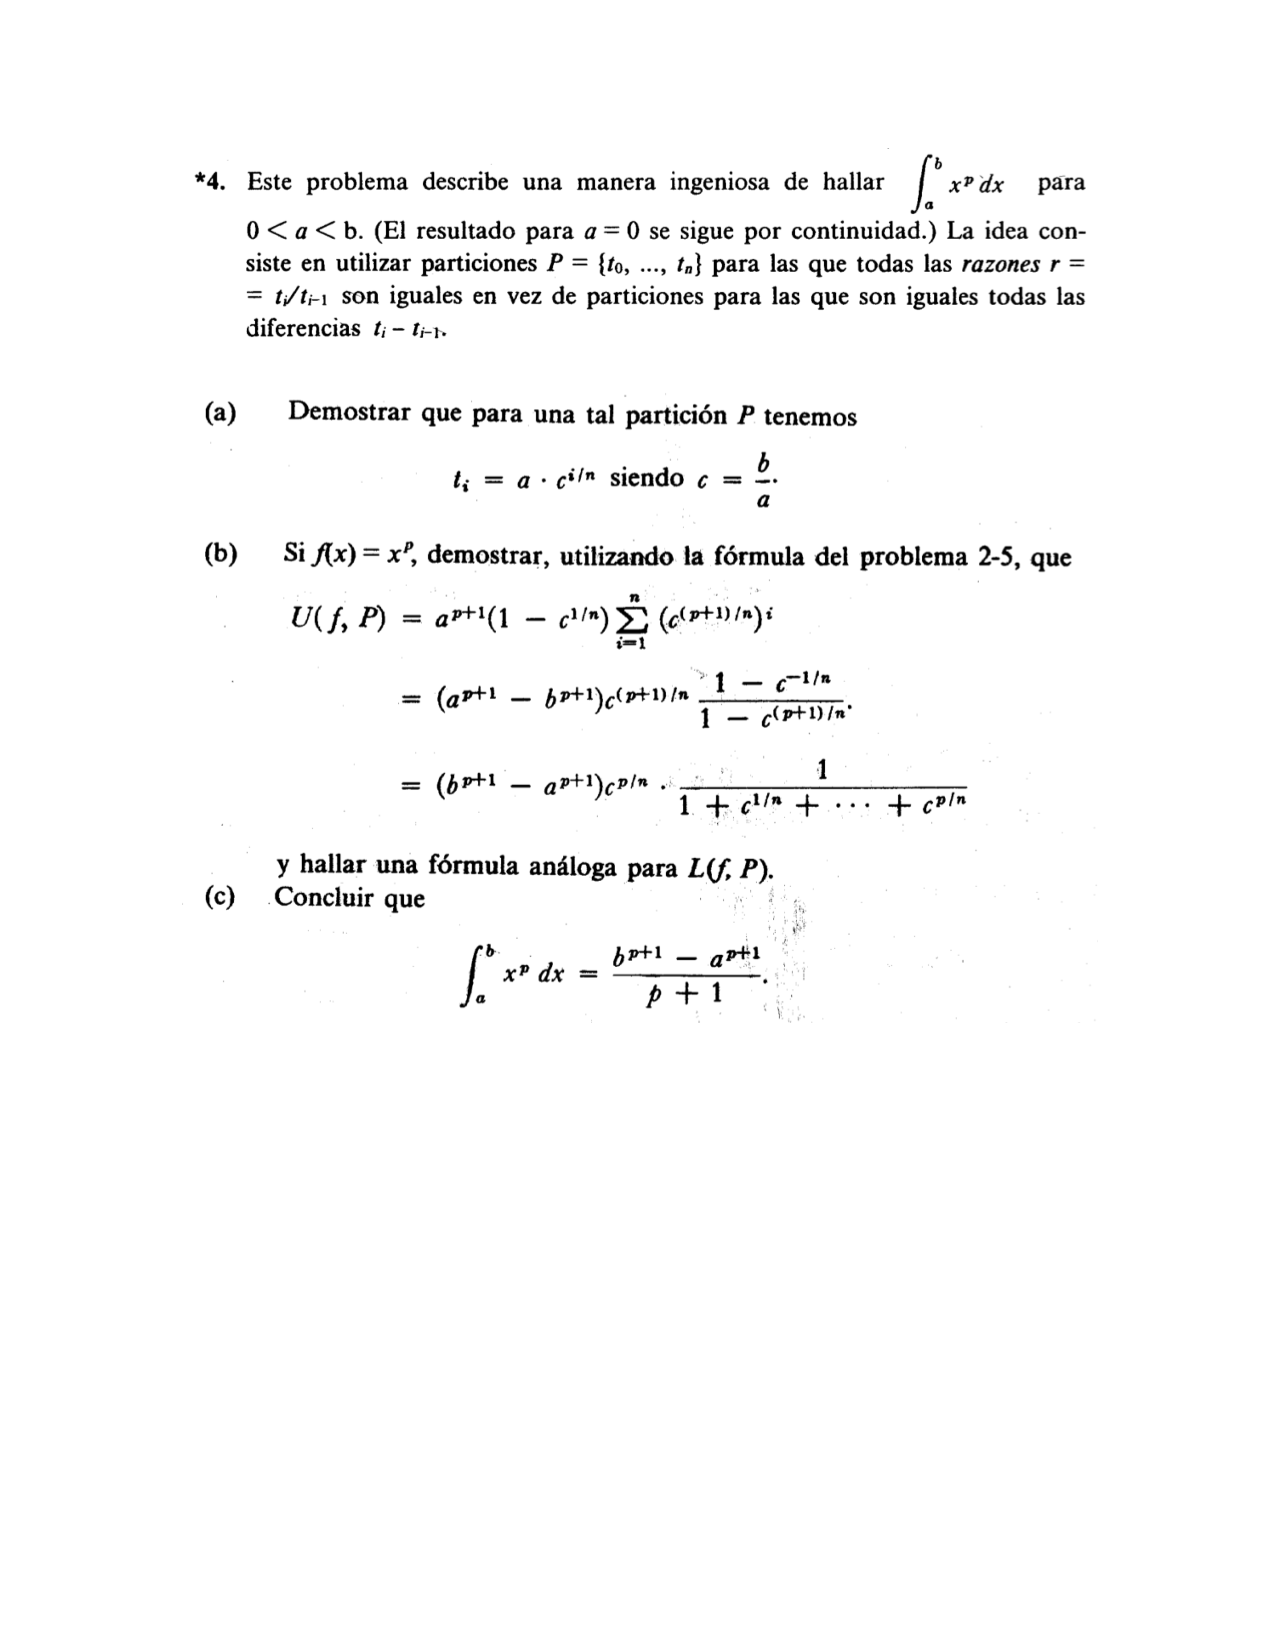
\includegraphics[width= 0.7 \linewidth, page = 1]{IMAGES/PORTADA/13-4-spivak.pdf}
\end{frame}
% )))

\section[Inciso A.]{Particiones.} % (((
% \frame{\sectionpage}
\begin{frame}[t]
	\frametitle{\secname}
	\begin{definition}
		Sean \(a,b \in \mathbb{R}\) con \(a<b\). \\ 
		Sea \(n \in \mathbb{N} ^ +\). \\ 
		Una \textbf{partición} \(P \subseteq \mathbb{R}\) de \([a,b]\),
		es un conjunto bien ordenado con \(n\) elementos,
		\(P = \{t_0, \;\ldots,\; t_n\}\), tal que \(t_0 = a\), \(t_n = b\).
	\end{definition}
	\begin{block}{\it Inciso a)}
		Sean \(a,b \in \mathbb{R}\), tales que \(0 < a < b\). \\
		Sea \(P = \{t_0, \;\ldots,\; t_n\}\) partición de \([a,b]\),
		tal que \(\forall i \leqslant n\),
		\(r = \dfrac{t_i}{t_{i-1}}\).
		\pause
		Probar que \(\forall i \leqslant  n\),
		\[
			t_i = a \cdot c ^ {i / n} \hspace{1cm} c = \dfrac{b}{a}
		\]
	\end{block}
\end{frame}

\begin{frame}[t,fragile]
	\frametitle{\secname}
	\textbf{Observación.} 
	Notar que la partición \(t_i = a \cdot c^{i/n}\) tiene sentido.
	\begin{itemize}
		\item \(t_0 = a \cdot c^0 = a\).
		\item \(t_n = a \cdot c ^ {n/n} = b\).
	\end{itemize}
	\pause
	\begin{center}
		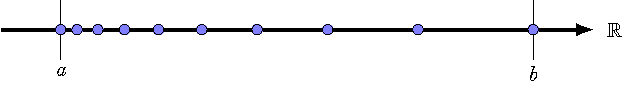
\includegraphics[width= \linewidth, page = 1]{IMAGES/1/1.pdf}
	\end{center}
	También observar que \(c = b/a > 1\). \\ \pause
	Así que \(t_{i+1} - t_i > t_i - t_{i-1}\), \(\forall i \leqslant n\). \pause
	\[
		\begin{array}{rcl}
			t_{i+1} - t_i & = & a \cdot c^ {(i+1) / n} - a \cdot c^ {i/n}
			\pause
			= c \cdot \Big[a \cdot c^ {i/n} - a \cdot c^ {(i-1) /n}\Big] \\[2mm]
			\pause
			& > & a \cdot c^ {i/n} - a \cdot c^ {(i-1) /n} \\[2mm] 
			\pause
			& = & t_{i} - t_{i-1} .
		\end{array}
	\]
\end{frame}

\begin{frame}[t,fragile]
	\frametitle{\secname}
	\textbf{Demostración.} Sean \(0 < a < b\). \\
	Sea \(P = \{t_0, \;\ldots,\; ,t_n\} \subseteq [a,b]\) tal que 
	\[
		t_0 = a \;,\; t_n = b
		\hspace{1cm},\hspace{1cm} r = \dfrac{t_i}{t_{i-1}}, \forall i \leqslant  n.
	\]
	\pause
	Entonces
	\[
		r^n = \dis\prod_{i=1}^{n} r \pause
		= \dis\prod_{i=1}^{n} \dfrac{t_i}{t_{i-1}} \pause
		= \dfrac{t_1}{t_0} \cdot \dfrac{t_2}{t_1} \cdot \dfrac{t_3}{t_2} \pause
		\;\cdots\; \dfrac{t_{n-1}}{t_{n-2}} \cdot \dfrac{t_n}{t_{n-1}} \pause
		= \dfrac{t_n}{t_0} \pause
		= \dfrac{b}{a} = c.
	\]
	Así, \(r = c^ {1/n}\). \pause
	Ahora, para \(i \leqslant n\),
	\[
		\dfrac{t_i}{t_0} = \pause
		\dis\prod_{k=1}^{i} \dfrac{t_k}{t_{k-1}} = \pause
		\dis\prod_{k=1}^{i} r = r^i = c^ {i/n}.
	\]
	Entonces
	\[
		t_i = t_0 \cdot c^ {i/n} = a \cdot c^ {i/n}. \qed
	\]
\end{frame}
% )))

\section[Inciso B.]{Suma Superior e Inferior.} % (((
% \frame{\sectionpage}
\begin{frame}[t,fragile]
	\frametitle{\secname}
	\begin{columns}[t]
		\column{0.55\textwidth}
\begin{definition}
	Sean \(a<b\).
	Sea \(P = \{t_0, \;\ldots,\; t_n\}\) \\ partición de \([a,b]\).
	Sea \(f : \mathbb{R} \longrightarrow \mathbb{R}\). 
	Definimos
	\[
		\begin{array}{rcl}
			m_i & = & \dis\inf f([t_{i-1} ,t_i]) \\[2mm]
			M_i & = & \dis\sup f([t_{i-1} ,t_i]) \\[2mm]
			\pause
			L(f,P) & = & \dis\suma_{i=1}^{n} m_i \cdot (t_i-t_{i-1}) \\[2mm]
			U(f,P) & = & \dis\suma_{i=1}^{n} M_i \cdot (t_i-t_{i-1})
		\end{array}
	\]
\end{definition}
\pause
		\column{0.35\textwidth}
	Usaremos fuertemente el sig. Lema.
	\begin{lemma}
		Sea \(n \in \mathbb{N}\). \\ 
		Sea \(x \in \mathbb{R}\), con \(x \ne 1\). \\ 
		\pause
		Entonces
		\[
			\dis\suma_{i=0}^{n} x ^ i = \dfrac{1-x^ {n+1}}{1-x}.
		\]
	\end{lemma}
	\pause
		Notar que la suma se inicia en \(i=0\).
	\end{columns}
\end{frame}

\begin{frame}[t,fragile]
	\frametitle{\secname}
	\begin{block}{\it Inciso b).}
		Sea \(p \in \mathbb{N}\).
		Sea \(f: \mathbb{R} \longrightarrow \mathbb{R}\), \(f(x) = x^p\). \\
		Sea \(P \subseteq [a,b]\) la partición definida anteriormente. \\ 
		\pause
		Prueba que
		\vspace{-5mm}
		\[
			\begin{array}{rcl}
				U(f,P) & = & a^ {p+1} (1- c^ {-1/n}) 
				\dis\suma_{i=1}^{n} \big(c^ {(p+1) /n}\big) ^ i\\[2mm]
				& = & (a^ {p+1} - b^ {p+1}) c^ {(p+1) /n} 
				\dfrac{1-c^ {-1/n}}{1-c^ {(p+1) /n}}\\[5mm]
				& = & (b^ {p+1} - a^ {p+1} ) c^ {p/n}
				\dfrac{1}{\dis\suma_{i=0}^{p} c^ {i/n}} .
			\end{array}
		\]
	\end{block}
\end{frame}

\begin{frame}[t,fragile]
	\frametitle{\secname}
	\textbf{Demostración.} \\
	Notar que
	\begin{itemize}
		\item \(r = c^ {1/n}\),
		\item \(t_i = a \cdot c^ {i/n} = a \cdot r ^ i\),
		\item \(f\) es cresciente. \pause
			Así que 
			\[
				M_i = \dis\sup f([t_{i-1} , t_i]) = t_i^p = (ar ^ i) ^ p = a ^ pr^ {ip}.
			\]
		\item Calculemos \(t_i - t_{i-1}\).
			\pause
			\[
				t_i-t_{i-1} = ar ^ i - ar^ {i-1} \pause
				= ar ^ i (1 - r^ {-1}).
			\]
	\end{itemize}
	\[
		U(f,P) = \dis\suma_{i=1}^{n} M_i \cdot (t_i-t_{i-1}) 
		= \dis\suma_{i=1}^{n} a ^ p r ^ {ip}  \cdot ar ^ i (1-r^ {-1}) =
	\]
\end{frame}

\begin{frame}[t,fragile]
	\frametitle{\secname}
	\[
		\begin{array}{rcl}
			& = & \dis\suma_{i=1}^{n} a ^ pr ^ {ip} \cdot ar ^ i (1-r^ {-1}) \\[8mm]
		\pause
			& = & a^ {p+1} (1-r^ {-1}) \dis\suma_{i=1}^{n} r^ {ip} r ^ i \\[8mm]
		\pause
			& = & a^ {p+1} (1-r^ {-1}) \dis\suma_{i=1}^{n} r^ {ip + i} \\[8mm]
		\pause
			& = & a^ {p+1} (1-r^ {-1}) \dis\suma_{i=1}^{n} r^ {i(p+1)} \\[8mm]
		\end{array}
	\]
\end{frame}

\begin{frame}[t,fragile]
	\frametitle{\secname}
	\[
		\begin{array}{rcl}
			& = & a^ {p+1} (1-r^ {-1}) \dis\suma_{i=1}^{n} r^ {i(p+1)} \\[8mm]
			\pause
			& = & a^ {p+1} (1-r^ {-1})
			\dis\suma_{i=1}^{n} \big(r^ {p+1}\big) ^ i \\[8mm] 
			\pause
			& = & a^ {p+1} (1-r^ {-1}) \Bigg[-1 + 
			\dis\suma_{i=0}^{n} \big(r^ {p+1}\big) ^ i\Bigg] \\[8mm]
			\pause
			& = & a^ {p+1} (1-r^ {-1}) \Bigg[-1 + 
			\dfrac{1- r^ {(p+1) (n+1)}}{1-r^ {p+1}}\Bigg]
		\end{array}
	\]
\end{frame}

\begin{frame}[t,fragile]
	\frametitle{\secname}
	\[
		\begin{array}{rcl}
			& = & a^ {p+1} (1-r^ {-1}) \Bigg[-1 + 
			\dfrac{1- r^ {(p+1) (n+1)}}{1-r^ {p+1}}\Bigg] \\[8mm]
			\pause
			& = & a^ {p+1} (1- r^ {-1}) \cdot 
			\dfrac{r^ {p+1} -1 + 1 - r^ {(p+1) (n+1)}}{1 -r^ {p+1}}\\[8mm]
			\pause
			& = & a^ {p+1} (1-r^ {-1}) 
			\dfrac{r^ {p+1} - r^ {(p+1) n} \cdot r^ {p+1}}{1- r^ {p+1}} \\[8mm]
			\pause
			& = & a^ {p+1} (1-r^ {-1}) r^ {p+1} 
			\dfrac{1 - r^ {(p+1) n}}{1-r^ {p+1}}
		\end{array}
	\]
\end{frame}

\begin{frame}[t,fragile]
	\frametitle{\secname}
	\[
		\begin{array}{rcl}
			& = & a^ {p+1} (1-r^ {-1}) r^ {p+1} 
			\dfrac{1 - r^ {(p+1) n}}{1-r^ {p+1}} \\[8mm] 
			\pause
			& = & a^ {p+1} (1-r^ {(p+1) n}) r^ {p+1} 
			\dfrac{1 - r^ {-1}}{1- r^ {p+1}}
		\end{array}
	\]
	\pause
	Notar que \(r^ {(p+1) n} = \pause
	(c^ {1/n})^ {(p+1) n} = \pause
	c^ {(p+1) n /n} = \pause
	c^ {p+1} = \pause
	\left(\dfrac{b}{a} \right)^ {p+1}\). \\ 
	\pause
	Entonces
	\[
		\begin{array}{rcl}
			U(f,P) & = & (a^ {p+1} - b^ {p+1}) r^ {p+1} \cdot 
			\dfrac{1 - r^ {-1}}{1- r^ {p+1}} \\[8mm]
			\pause
			& = &  (a^ {p+1} - b^ {p+1}) r^ {p} \cdot 
			\dfrac{r - 1}{1 - r^ {p+1}}
		\end{array}
	\]
\end{frame}

\begin{frame}[t,fragile]
	\frametitle{\secname}
	\[
		\begin{array}{rcl}
			& = &  (a^ {p+1} - b^ {p+1}) r^ {p} \cdot 
			\dfrac{r - 1}{1 - r^ {p+1}}\\[8mm]
			\pause
			& = & (b^ {p+1} - a^ {p+1}) r ^ p \cdot 
			\dfrac{1-r}{1-r^ {p+1}}\\[8mm]
			\pause
			& = & (b^ {p+1} - a^ {p+1}) r ^ p\cdot 
			\dfrac{1}{\dis\suma_{i=0}^{p} r ^ i} \\[1.2cm] 
			\pause
			& = & r ^ p \cdot 
			\dfrac{b^ {p+1} - a^ {p+1}}{\dis\suma_{i=0}^{p} r ^ i}. \qed
		\end{array}
	\]
\end{frame}

\begin{frame}[t,fragile]
	\frametitle{\secname}
	\begin{block}{\it Inciso b)}
		Encontrar una fórmula análoga para \(L(f,P)\).
	\end{block}
	\textbf{Solución.} Recordar que
	\begin{itemize}
		\item \(M_i = t_i ^ p \pause
			= (ar ^ i) ^ p \pause
			= a ^ p r^ {ip}\).
		\item \(m_i = \dis\inf f([t_{i-1},t_i]) \).
		\item \(L(f,P) = \dis\suma_{i=1}^{n} m_i \cdot (t_i-t_{i-1})\).
	\end{itemize}
	Como \(f\) es cresciente, \vspace{-3mm}
	\[
		m_i =
	 t_{i-1} ^ p = \pause
	 (a \cdot r ^ {i-1} ) ^ p = \pause
	 a ^ p \cdot r^ {(i-1) p} = \pause
	 a ^ p r^ {ip} \cdot r^ {-p} = \pause
	 M_i \cdot r^ {-p}.
	\]
	Por tanto \(
	L(f,P) 
	= \dis\suma_{i=1}^{n} M_i \cdot r^ {-p} \cdot (t_i-t_{i-1}) \pause
	= r^ {-p} \cdot U(f,P)\).
\end{frame}

\begin{frame}[t,fragile]
	\frametitle{\secname}
	Hemos probado que
	\[
		U(f,P) = (b^ {p+1} - a^ {p+1}) r ^ p \cdot 
		\dfrac{1}{\dis\suma_{i=0}^{p} r ^ i}.
	\]
	Entonces
	\[
		\begin{array}{rcl}
			L(f,P) & = & r^ {-p} \cdot U(f,P) \\[2mm]
			& = & r^ {-p} (b^ {p+1} - a^ {p+1}) r ^ p \cdot 
			\dfrac{1}{\dis\suma_{i=0}^{p} r ^ i} \\[8mm]
			& = & \dfrac{b^ {p+1} - a^ {p+1}}{\dis\suma_{i=0}^{p} r^ i}. \qed
		\end{array}
	\]
\end{frame}
% )))

\section[Inciso C.]{Integral de \(f\).} % (((
% \frame{\sectionpage}
\begin{frame}[t]
	\frametitle{\secname}
	\begin{block}{Inciso c)}
		Probar que \(\dis\int _a ^ b f \; = \dfrac{b^ {p+1} - a^ {p+1}}{p+1}\).
	\end{block}
	\pause
	\textbf{Demostración.} 
	Recordar que para \(x >0\),
	\[
		\dis\lim_{n\rightarrow \infty} x^ {1/n} = 1.
	\]
	Aplicaremos este resultado a \(r_n = c^ {1/n} \pause
	= \left(\dfrac{b}{a} \right)^ {1/n}\). \\ 
	Hemos probado que
	\[
		L(f,P_n) = \dfrac{b^ {p+1} - a^ {p+1}}{\dis\suma_{i=0}^{p} r_n ^ i},
		\hspace{1cm} 
		U(f,P_n) = r_n^ p \cdot 
		\dfrac{b^ {p+1} - a^ {p+1}}{\dis\suma_{i=0}^{p} r_n^i}.
	\]
\end{frame}

\begin{frame}[t,fragile]
	\frametitle{\secname}
	Notamos que
	\vspace{-2mm}
	\[
		\dis\lim_{n\rightarrow \infty} L(f,P_n) \leqslant 
		\dis\sup _P L(f,P) \leqslant \dis\inf _P U(f,P) \leqslant 
		\dis\lim_{n\rightarrow \infty} U(f,P_n).
		\vspace{-3mm} 
	\]
	Y además
	\vspace{-4mm}
	\[
		\begin{array}{rcl}
			\dis\lim_{n\rightarrow \infty} L(f,P_n) = \dis\lim_{n\rightarrow \infty} 
			\dfrac{b^ {p+1} - a^ {p+1}}{\dis\suma_{i=0}^{p} r_n ^ i}
			& = & \dfrac{b^ {p+1} - a^ {p+1}}{\dis\suma_{i=0}^{p} 
			\big(\dis\lim_{n\rightarrow \infty} r_n\big) ^ i} \\[1.5cm]
			& = & \dfrac{b^ {p+1} - a^ {p+1}}{
				\dis\suma_{i=0}^{p} 1} \\[1.4cm]
			& = & \dfrac{b^ {p+1} - a^ {p+1}}{p+1}.
		\end{array}
	\]
\end{frame}

\begin{frame}[t,fragile]
	\frametitle{\secname}
	Además, como \(L(f,P_n) = r_n^ {-p} \cdot U(f,P_n)\), \pause
	entonces
	\[
		\begin{array}{rcl}
		\dis\lim_{n\rightarrow \infty} U(f,P_n) = 
		\dis\lim_{n\rightarrow \infty} r_n^ p \cdot L(f,P_n)
		& = & (\dis\lim_{n\rightarrow \infty} r_n ^ p) \cdot
		(\dis\lim_{n\rightarrow \infty} L(f,P_n)) \\[4mm]
		& = & 1 \cdot 
		\dfrac{b^ {p+1} - a^ {p+1}}{p+1} .
		\end{array}
	\]
	Así,
	\[
		\dis\int _a ^ b f \; = 
		\dfrac{b^ {p+1} - a^ {p+1}}{p+1}. \qed
	\]
\end{frame}
% )))

\end{document}
